%%%%%%%%%%%%
% ABSTRACT %
%%%%%%%%%%%%
\abstract{Numerical Weather Prediction (NWP) models produce forecasts that, although improve continuously in reliability/skill, represent an average over the model grid-box. For some applications, users require forecasts at specific locations instead. Forecasters can add value to model predictions issued for smaller scales than the model resolution as they understand model biases/errors, interpret how they might impact the weather at a location, and summarize the information to users. However, forecasters call upon past model performance experience, which can take years to build up, it is no easily adaptable to new model versions, and it might generate biased forecasts. A novel statistical post-processing methodology (ecPoint) that produces more reliable/skilful probabilistic forecasts at points can also help forecasters to overcome the challenges mentioned earlier. The formulation of ecPoint probabilities does not depend on personal experience. They are based on a global observational database instead. ecPoint probabilities adapt quickly to biases/errors in new model versions thanks to a dynamic calibration process. Finally, ecPoint summarizes in one intelligible probability distribution the complex raw probabilistic information. Thus, forecasters do not have to do it themselves. However, ecPoint adds layers of complexity to traditional probabilistic ensemble-based forecasts (PEFs). Could current standard PEFs training be sufficient to make forecasters fully appreciate ecPoint potentialities and adopt it in operational environments? A one-year trial with two different users showed that ecPoint-tailored training must be provided to improve the understanding of ecPoint forecasts, no matter what is the previous experience of forecasters with PEFs. Therefore, this study defines guidelines to communicate ecPoint forecasts to users better.}


%%%%%%%%%%%%%%%%%%%%%%
% MAIN BODY OF PAPER %
%%%%%%%%%%%%%%%%%%%%%%
\begin{document}
\maketitle



%%%%%%%%%%%%%%%%%%%%
% Results
\section{Results}

\subsubsection{Subjective Verification}

\begin{figure}
\centerline{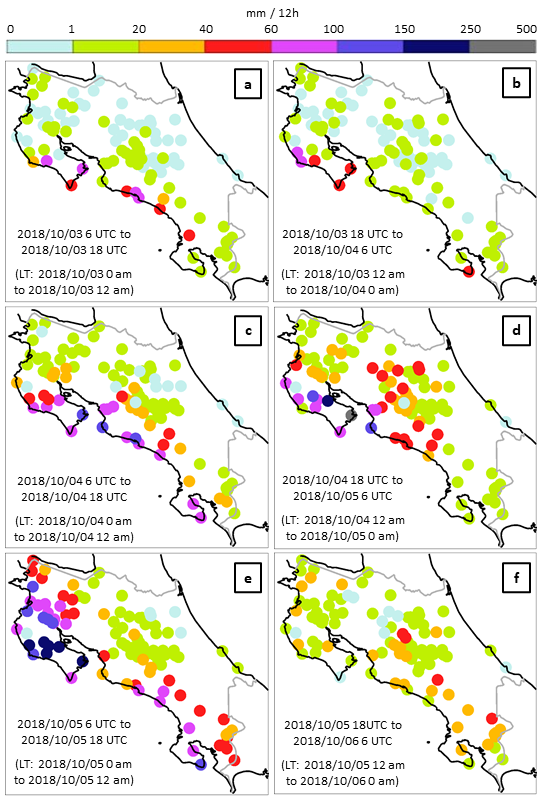
\includegraphics[width=19pc]{manuscript/Figures/Results_Obs_CaseStudy_CR.png}}
\caption{Panel (a) shows the climate regions of Costa Rica defined by IMN. Panels from (a) to (f) show 12-hourly rainfall observations during the extreme rainfall event occurred between October 3rd and 5th, 2018.}
\label{Obs_CaseStudy_CR}
\end{figure}

\begin{figure*}
\centerline{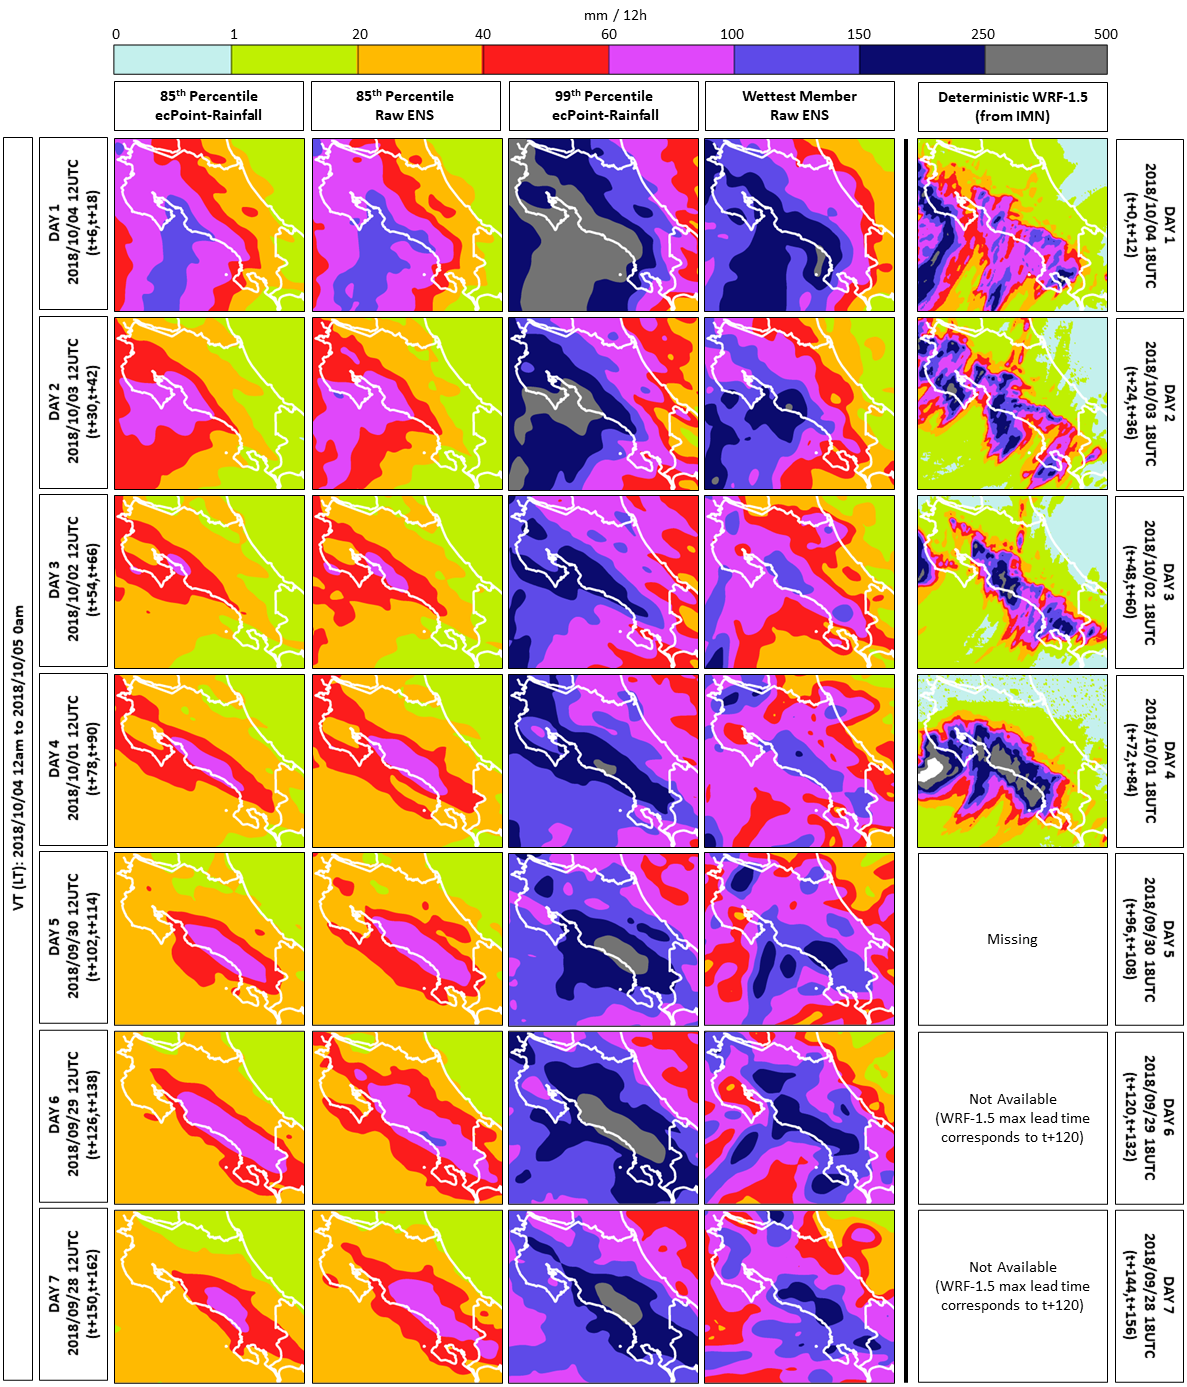
\includegraphics[width=39pc]{manuscript/Figures/Results_CaseStudy_Comparison_Models_CR.png}}
\caption{Forecast evolution (from day 7 to day 1) for the rainfall event occurred between October 4th at 12am and October 5th at 0am (see Fig.\ref{Obs_CaseStudy_CR}d to compare the forecasts with the observations). From the left, the first column shows the 85th percentile for ecPoint-Rainfall (as used operationally by IMN), the second column shows the 85th percentile for the raw ENS, the third column shows the 99th percentile for ecPoint-Rainfall, the fourth column shows the wettest member of the raw ENS, and the fifth column shows the deterministic forecast from WRF-1.5 (spatial resolution of 1.5 km) typically used by IMN in the forecasts of extreme localized rainfall events. The shown raw ECMWF ENS and ecPoint-Rainfall forecasts correspond to runs at 12 UTC, which is the first available run from Europe to IMN forecasters due to time difference between Europe and America (UTC-6). The displayed WRF-1.5 forecasts correspond to runs at 18 UTC, which is the first run available to IMN forecasters in the morning for their in-house models. The colour scheme of the second column plots have been modified, compared to the original IMN products (see Fig.\ref{ecPoint_Product_CR}d), to standardize all the plots in this figure, and make easier the forecasts comparison between models.}
\label{Results_CaseStudy_Comparison_Models_CR}
\end{figure*}




\subsection{"Offline phase": IMN}

\begin{figure}
\centerline{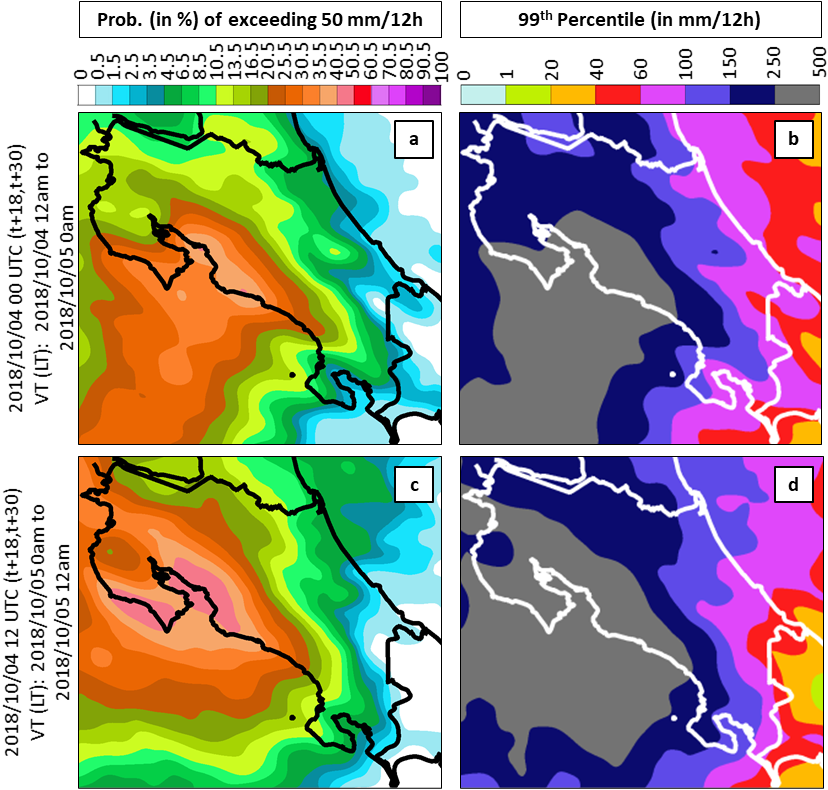
\includegraphics[width=19pc]{manuscript/Figures/Results_CaseStudy_Comparison_Prob_Perc.png}}
\caption{Panels (a) and (c) show the probabilities of not exceeding 50 mm/12h, and panels (b) and (d) show the 99th percentile, both for ecPoint-Rainfall forecasts. Panels (a) and (b) correspond to the forecast on 2018/10/04 at 00 UTC (t+18,t+30), which correspond to the period between 2018/10/04 12am and 201/10/05 0am (local time). Panels (c) and (d) correspond to the forecast on 2018/10/04 at 12 UTC (t+18,t+30), which correspond to the period between 2018/10/05 0am and 201/10/05 12am (local time).} 
\label{CaseStudy_Comparison_Prob_Perc}
\end{figure}

\begin{figure}
\centerline{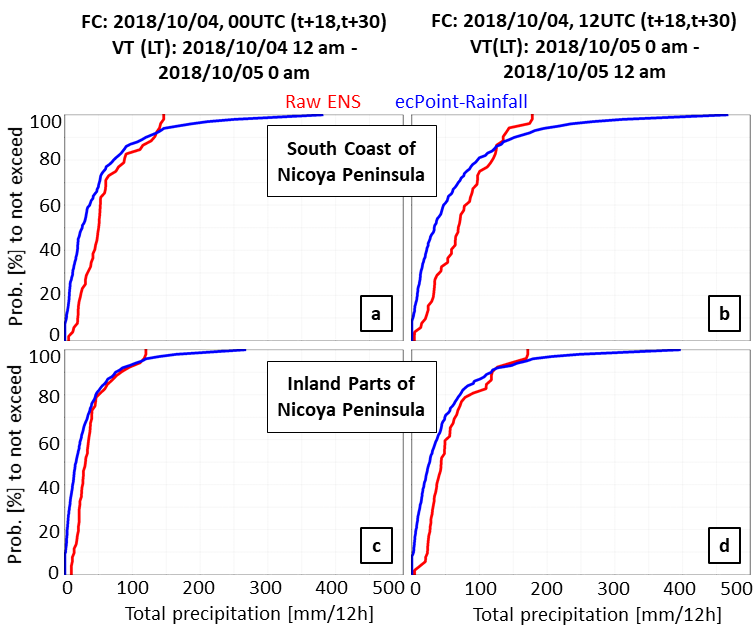
\includegraphics[width=19pc]{manuscript/Figures/Results_CaseStudy_CDFs_CR.png}}
\caption{CDFs for ecPoint-Rainfall (in blue) and raw ENS (in red). Panels (a) and (b) display the CDFs for a location representative of the south coast of the Nicoya peninsula (lat=9.82,lon=-84.94). Panels (c) and (d) display the CDFs for a location representative of the inland parts of the Nicoya peninsula (lat=10.08,lon=-85.47). Panel (a) and (c) correspond to the forecast on 2018/10/04 at 00 UTC (t+18,t+30), which correspond to the period between 2018/10/04 12am and 201/10/05 0am (local time). Panel (b) and (d) correspond to the forecast on 2018/10/04 at 12 UTC (t+18,t+30), which correspond to the period between 2018/10/05 0am and 201/10/05 12am (local time).}
\label{Results_CaseStudy_CDFs_CR}
\end{figure}


\subsection{"Offline phase": OMSZ}


\subsection{Revised ecPoint-Rainfall guidelines}

\begin{figure*}
\centerline{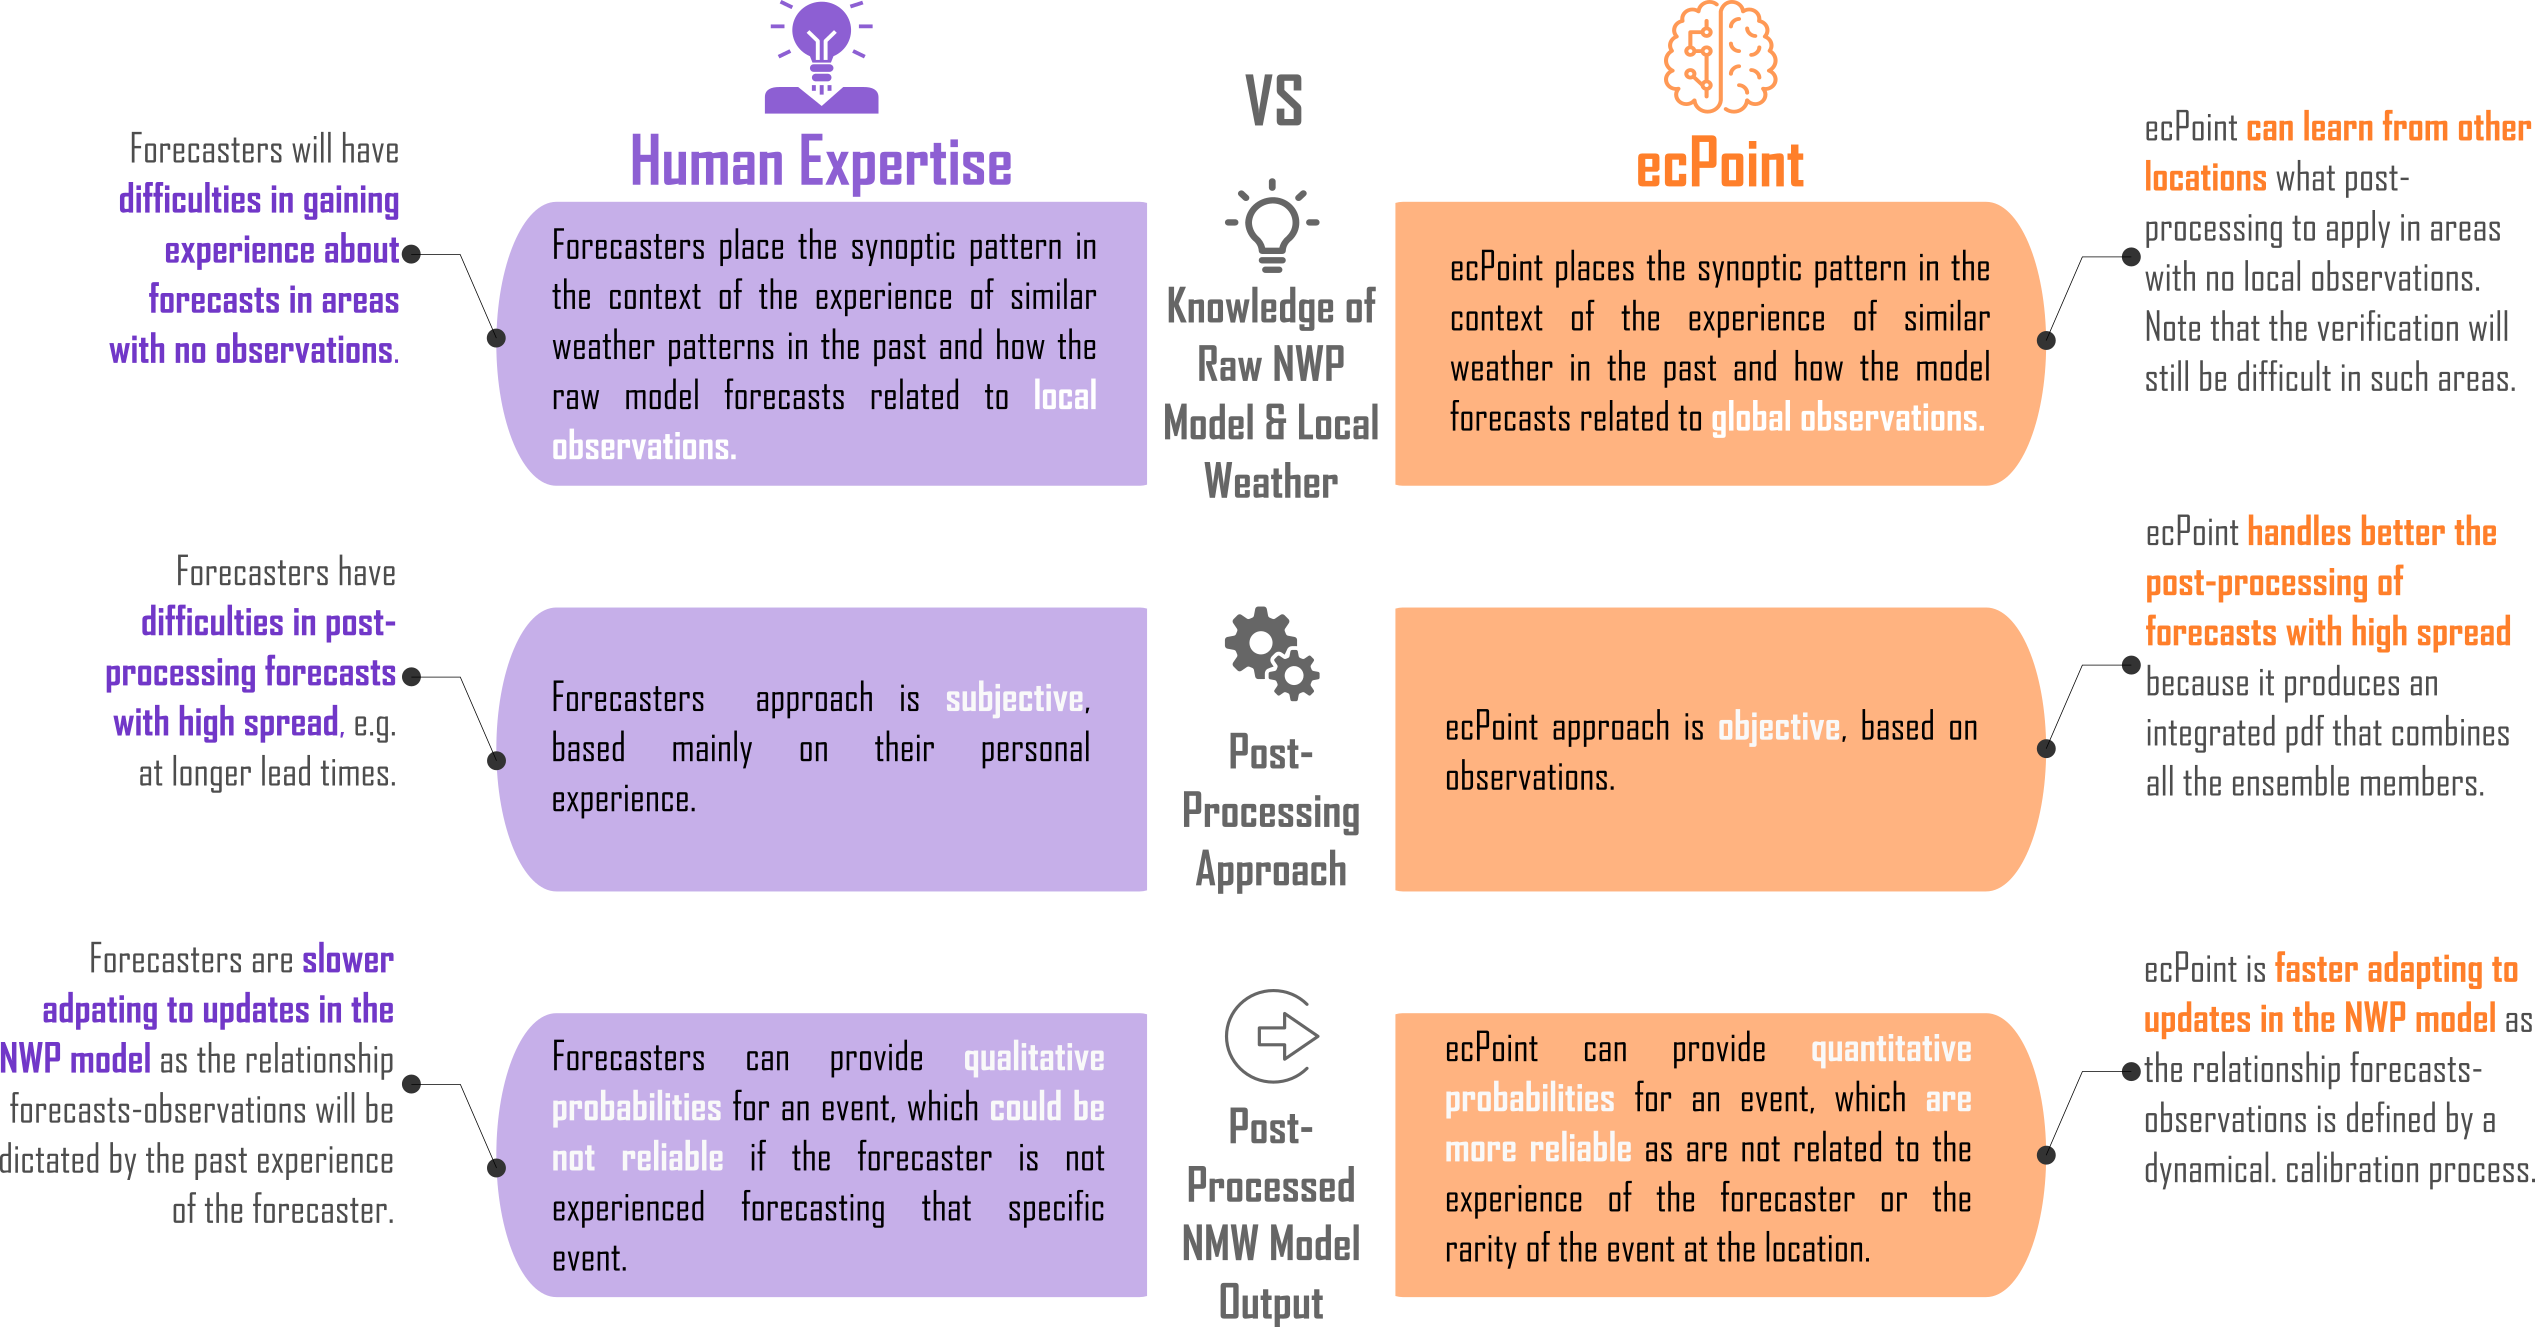
\includegraphics[width=39pc]{manuscript/Figures/Results_Correlation_Forecasters_ecPoint.png}}
\caption{Comparison between the forecasters approach when building their mental model during the forecast creation process, and the ecPoint post-processing methodology.}
\label{Results_Correlation_Forecasters_ecPoint}
\end{figure*}





IMN evaluated the ecPoint-Rainfall guidance for the selected event from short (day 1) to medium (day 7) lead times employing the product they developed during the trial (see Fig.\ref{Fig3}). Only 12 UTC runs were analyzed as those are the only ones used at IMN for daily warnings given the time difference between Europe and Central America (UTC-6). IMN’s own conclusions can be summarized in three main points:

\begin{enumerate}
\item ecPoint-Rainfall predicted well the beginning and the end of the rainfall event in every run from September 27th.
\item On October 4th, ecPoint-Rainfall identified Región Pacifico Central and Pacifico Sur as the most impacted areas, underestimating the rainfall amounts in Región Pacifico Norte especially in the Nicoya peninsula where totals of up to 400mm/24h were observed. No runs reached such totals. Only the run on October 4th predicted values higher than 100 mm/12h.”
\item Most runs [based on the 85th percentile of ecPoint-Rainfall] predicted with one day of delay [October 5th] the wettest day which was on October 4th.
\end{enumerate}

\begin{figure*}
\centerline{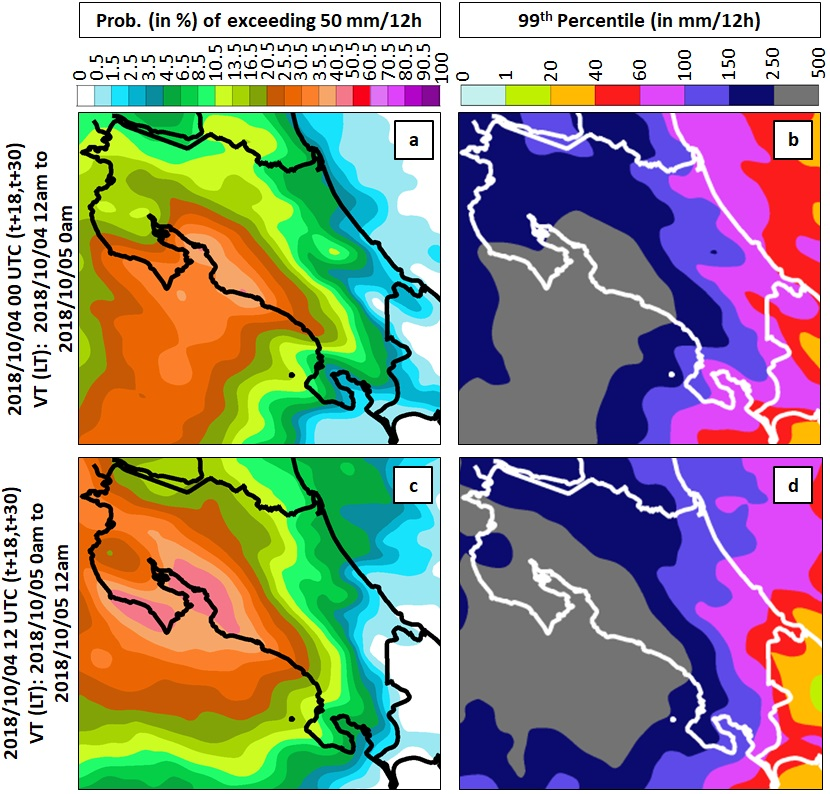
\includegraphics[width=39pc]{manuscript/Figures/Fig5.jpg}}
\caption{Panel (a) shows the climate regions of Costa Rica defined by IMN. Panels from (o-1) to (o-6) show 12-hourly rainfall observations between October 3rd and 5th, 2018. Panels from (i-1) to (i-3) show the impacts caused by the extreme event in the regions in which CNE declared the state of red alert (the photos come from www.teletica.com).}
\label{Fig5}
\end{figure*}


\subsection{Results from the trial}
The results from the trial are described in Table \ref{Table1}. It contains (1) a description of products created at IMN and OMSZ from ecPoint-Rainfall, (2) a description of the verification case study selected by the two meteorological services, and (3) the forecasters comments about the performance of the new post-processed rainfall forecasts in predicting the analyzed extreme rainfall events.

\subsection{Results from the dialogue with the forecasters}

\subsubsection{IMN: On the selection of ecPoint-Rainfall's 85th percentile to predict extreme localized rainfall}

\begin{figure}
\centerline{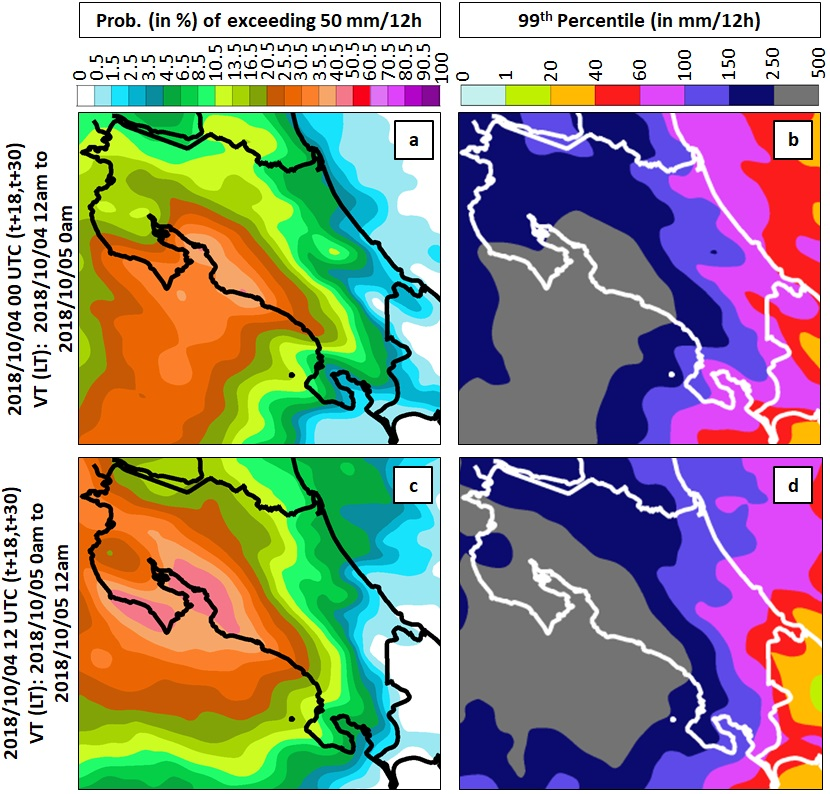
\includegraphics[width=19pc]{manuscript/Figures/Fig6.jpg}}
\caption{Panels (a) and (c) show the probabilities of not exceeding 50 mm/12h, and panels (b) and (d) show the 99th percentile, both for ecPoint-Rainfall forecasts. Panels (a) and (b) correspond to the forecast on 2018/10/04 at 00 UTC (t+18,t+30), which correspond to the period between 2018/10/04 12am and 201/10/05 0am (local time). Panels (c) and (d) correspond to the forecast on 2018/10/04 at 12 UTC (t+18,t+30), which correspond to the period between 2018/10/05 0am and 201/10/05 12am (local time).} 
\label{Fig6}
\end{figure}

IMN reported that the 85th percentile was selected to predict extreme events but to not focus only on the \textit{"worst-case scenarios"}. IMN forecasters pointed out, for example, that events around 50 mm/12h can already cause some impacts on the Pacific coast of Costa Rica or in the capital city, San José. Such events are relatively frequent in Costa Rica. Therefore, IMN forecasters thought they would miss such more frequent events if they look only at the highest percentiles. \par
IMN assessment is fair. On the other hand, by looking only at the 85th percentile (which would forecast events that have, on average, a 1 in 7 chance to occur), forecasters would miss the opportunity to be aware of what could be the possible "worst-case scenario". The latter becomes, indeed, a piece of vital information when preparing forecasts for critical decision-making processes in highly uncertain weather scenarios like the one analyzed. \par
During the dialogue with IMN forecasters, it was discussed the possibility to make available to forecasters the probabilities of exceeding a certain threshold. For example, 50 mm/12h is a rainfall event that can generate some impacts in some areas of Costa Rica. Forecasters could display on a map-plot the probabilities of exceeding 50 mm/12h (see mock-up product in Fig.\ref{Fig5}a and c) and identify whether in the concerning areas the probabilities of exceeding 50 mm/12h are higher than a probability threshold previously defined by IMN for which action needs to be taken. At the same time, by looking at the 99th percentile (see mock-up product in Fig.\ref{Fig5}b and d), forecasters could identify those areas at risk of being affected by the "worst-case scenario" (as it represents those events with, on average, a 1 in 100 chance to occur), and provide a richer warning on the areas at risk of highest impacts. \par
When both products (Fig.\ref{Fig5}) were shown to IMN forecasters forecasters to see whether they would have reformulated their forecasts for the case study, they produced a much more aware warning about the areas at risk of highest impacts (like those in https://www.imn.ac.cr/es/web/imn/avisos-meteorologicos). \par
Furthermore, subsequent examination of different extreme rainfall cases around the world has shown that raw ENS and ecPoint-Rainfall’s CDFs tend to cross around the 85th percentile, and ECMWF users might not extract extra information from ecPoint-Rainfall not provided by the raw ENS.


\subsubsection{IMN: On the underestimation of the rainfall values in the Nicoya peninsula.}

\begin{figure*}
\centerline{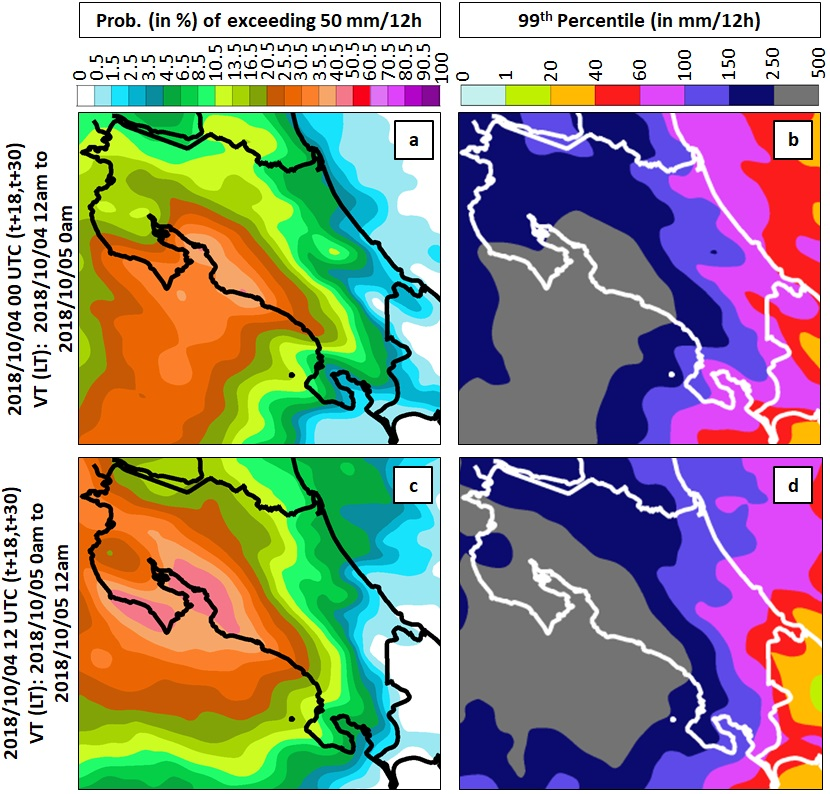
\includegraphics[width=39pc]{manuscript/Figures/Fig7.jpg}}
\caption{Forecast evolution (from day 7 to day 1) for the rainfall event occurred between October 04th at 12am and October 5th at 0am (see Fig. \ref{Fig4}o-4 to compare the forecasts with the observations). From the left, the first column shows the 85th percentile for ecPoint-Rainfall, the second column shows the 85th percentile for the raw ENS, the third column shows the 99th percentile for ecPoint-Rainfall, the fourth column shows the wettest member of the raw ENS, and the fifth column shows the deterministic forecast from WRF-1.5 provided by IMN (spatial resolution of 1.5 km). The shown raw ECMWF ENS and ecPoint-Rainfall forecasts correspond to runs at 12 UTC, which is the first available run from Europe to IMN forecasters due to time difference (UTC-6) between Europe and America. The displayed WRF-1.5 forecasts correspond to runs at 18 UTC, which is the first run available to IMN forecasters in the morning for their in-house models.}
\label{Fig7}
\end{figure*}

The observed rainfall patterns between October 3rd and 5th typify low-probability high-impact events, which might show high spatial variability of rainfall totals, including very localized extremes. To provide guidance for such events, IMN reported that \textit{"para estudiar la posibilidad de tener eventos extremos en determinada región o en dada circunstancia nos basamos en los acumulados de lluvia que  el modelo determinístico indique, la experiencia de los pronosticadores (sustentada también con investigación científica), la naturaleza del fenómeno que nos afecte (no produce el mismo impacto un frente frío que una onda tropical) y el estado de las regiones más vulnerables del país (por ejemplo, si ha estado lloviendo en días previos y hay cuencas saturadas".} [translation: to study the possibility of having extreme events in a certain region or in given circumstances, we rely on the accumulated rainfall that the deterministic model indicates, the experience of forecasters (also supported by scientific research), the nature of the phenomenon affecting us (a cold front does not produce the same impact of a tropical wave) and the state of the most vulnerable regions of the country (for example, if it has been raining in previous days and catchments are saturated.]. Furthermore, IMN forecasters stated that they would not use a global ensemble to predict such extreme events due to their coarse spatial resolution and difficulties parametrizing convective systems. IMN included ecPoint-Rainfall in the "global ensembles category" as the forecasts were provided on the same grid of the raw ENS. Such an approach indicates that a vital information to convey to users is that, although ecPoint-Rainfall and raw ENS are provided with the same grid resolution, they do not refer to the same spatial scale. In this instance, it appears that the usage guidelines provided by ECMWF did not fully meet this requirement. In future, it will be imperative to emphasized that the raw ENS (as any other NWP model) provides rainfall averages over the grid-box and ecPoint-Rainfall provides point-wise probabilistic rainfall forecasts at a location within a grid-box, even though ecPoint-Rainfall does not provide any information on where that point is within the grid-box. \par
Therefore, the post-processing technique aims to anticipate sub-grid variability and provide a wider distribution of equiprobable values that ideally captures in its tail those extreme events typically missed by global models. For this reason, ecPoint-Rainfall is particularly useful to providing guidance for events like those occurred in Costa Rica at the beginning of October. However, as explained in the previous section, such extreme events have a low probability of occurrence, and using a product based on the 85th percentile (~ 1 in 7 chance) suggests that ECMWF did not convey properly the message that percentiles below the 95th (1 in 20 chance) are usually not so well suited to providing guidance on low-probability high-impact events. During the dialogue with the forecasters, it was recommended to use the 98th (1 in 50 chance) or the 99th (1 in 100 chance) percentile to identify the areas at most risk of extreme localized rainfall. \par
Fig.~\ref{Fig6} shows the forecasts, up to day 7, for the rainfall event between midday October 4th and midnight October 5th (compare with observations in Fig.\ref{Fig4}o-4). The first and the second column in Fig.~\ref{Fig6} show, respectively, the 85th percentile of ecPoint-Rainfall and raw ENS. The maps in these two columns show to the reader what it was previously stated about the similarity of the raw ENS and ecPoint-Rainfall's 85th percentile. The third, the fourth and the fifth column in Fig.~\ref{Fig6} show, respectively, the 99th percentile of ecPoint-Rainfall, the wettest ENS member, and the rainfall accumulations for the deterministic WRF-1.5 model. ecPoint-Rainfall provides from day 7 a more consistent guidance on the location of the areas at most risk of extreme rainfall, i.e. the whole Pacific coast (including the Nicoya peninsula), with a signal that becomes better defined from day 2 and shows forecast values of the same order as those observed. On the other hand, the raw ENS and the WRF-1.5 provide a noisier and jumpier signal. In the raw ENS the Nicoya peninsula is not highlighted in the guidance until day 2, and the rainfall extremes are underestimated of ~50\% also at day 1. 


\subsubsection{IMN: On the misplacement of the wettest day.}

\begin{figure}
\centerline{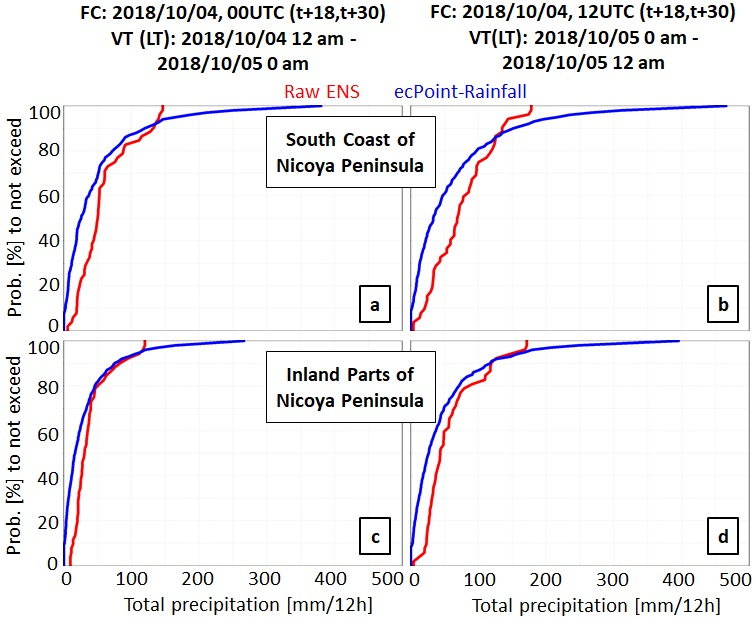
\includegraphics[width=19pc]{manuscript/Figures/Fig8.jpg}}
\caption{CDFs for ecPoint-Rainfall (in blue) and raw ENS (in red). Panels (a) and (b) display the CDFs for a location representative of the south coast of the Nicoya peninsula (lat=9.82,lon=-84.94). Panels (c) and (d) display the CDFs for a location representative of the inland parts of the Nicoya peninsula (lat=10.08,lon=-85.47). Panel (a) and (c) correspond to the forecast on 2018/10/04 at 00 UTC (t+18,t+30), which correspond to the period between 2018/10/04 12am and 201/10/05 0am (local time). Panel (b) and (d) correspond to the forecast on 2018/10/04 at 12 UTC (t+18,t+30), which correspond to the period between 2018/10/05 0am and 201/10/05 12am (local time).}
\label{Fig8}
\end{figure}

Examining the rainfall observations in Fig.~\ref{Fig4}o3-o5, the Nicoya peninsula appears, on average, wetter on October 5th than the previous day. Indeed, on October 4th more variable smaller rainfall totals were recorded, even though a local peak of 309.2 mm was observed in the south coast of the Nicoya peninsula (Fig.~\ref{Fig4}o-4). \par
The IMN approach of examining the 85th percentile of ecPoint-Rainfall to assess what was the possible wettest day for the whole event indicates that ECMWF should stress in its usage guidelines to not use only one percentile to identify the wettest day over a period of time. It was discussed with the IMN forecasters that, if provided with the whole rainfall distribution (i.e. the 99 percentiles), a better guideline would be to look at the whole CDF and identify, for different days, (1) the range of possible values given by the spread of the CDF, and (2) the shape of the distribution to identify what values are more likely (for example, a more vertical CDF indicates more confidence in the forecast). CDFs for the south coast (Fig.~\ref{Fig7}a-b) and inland parts (Fig.~\ref{Fig7}c-d) of the Nicoya peninsula for two different 12-hourly rainfall accumulations on October 4th (Fig.~\ref{Fig6}a-c) and 5th (Fig.~\ref{Fig7}b-d) are compared for ecPoint-Rainfall (in blue) and raw ENS (in red). The first thing to notice is that the raw ENS is providing a huge range of possible rainfall totals (at grid-scale) over the Nicoya peninsula on both days. However, because the area to the left of the raw ENS CDF (proportional to the ensemble mean) is bigger on October 5th for both coast and inland parts of the peninsula, forecasters might expect more rainfall on that day, instead of October 4th. On the other hand, the tails of the ecPoint-Rainfall CDFs tell the forecasters that both locations have the same probabilities, on both days, of experiencing much more extreme rainfall totals locally. \par
The guidance provided by the raw ENS and ecPoint-Rainfall could be supported by the observations. On the other hand, the recording of a higher local peak on October 4th instead of on October 5th can be a matter of chance, and it should not lead to the conclusion that that day was the wettest. Indeed, only part of the sub-grid scale variability of the precipitation field is known from observations. Denser observational networks would provide a better spatial representation of heavily affected areas, and they are considered vital for the evaluation of ecPoint-Rainfall in predicting extreme localized rainfall events, where heavy precipitation is observed in one location but not at neighbouring stations. Therefore, any deterministic statement about ecPoint-Rainfall placing correctly or not the wettest day within a period suggests that ECMWF needs to provide a better guidance on what is a better baseline when comparing ecPoint-Rainfall against point observations.


%%%%%%%%%%%%%%%%%%%%
% Discussions
\section{Discussions}

\begin{figure*}
\centerline{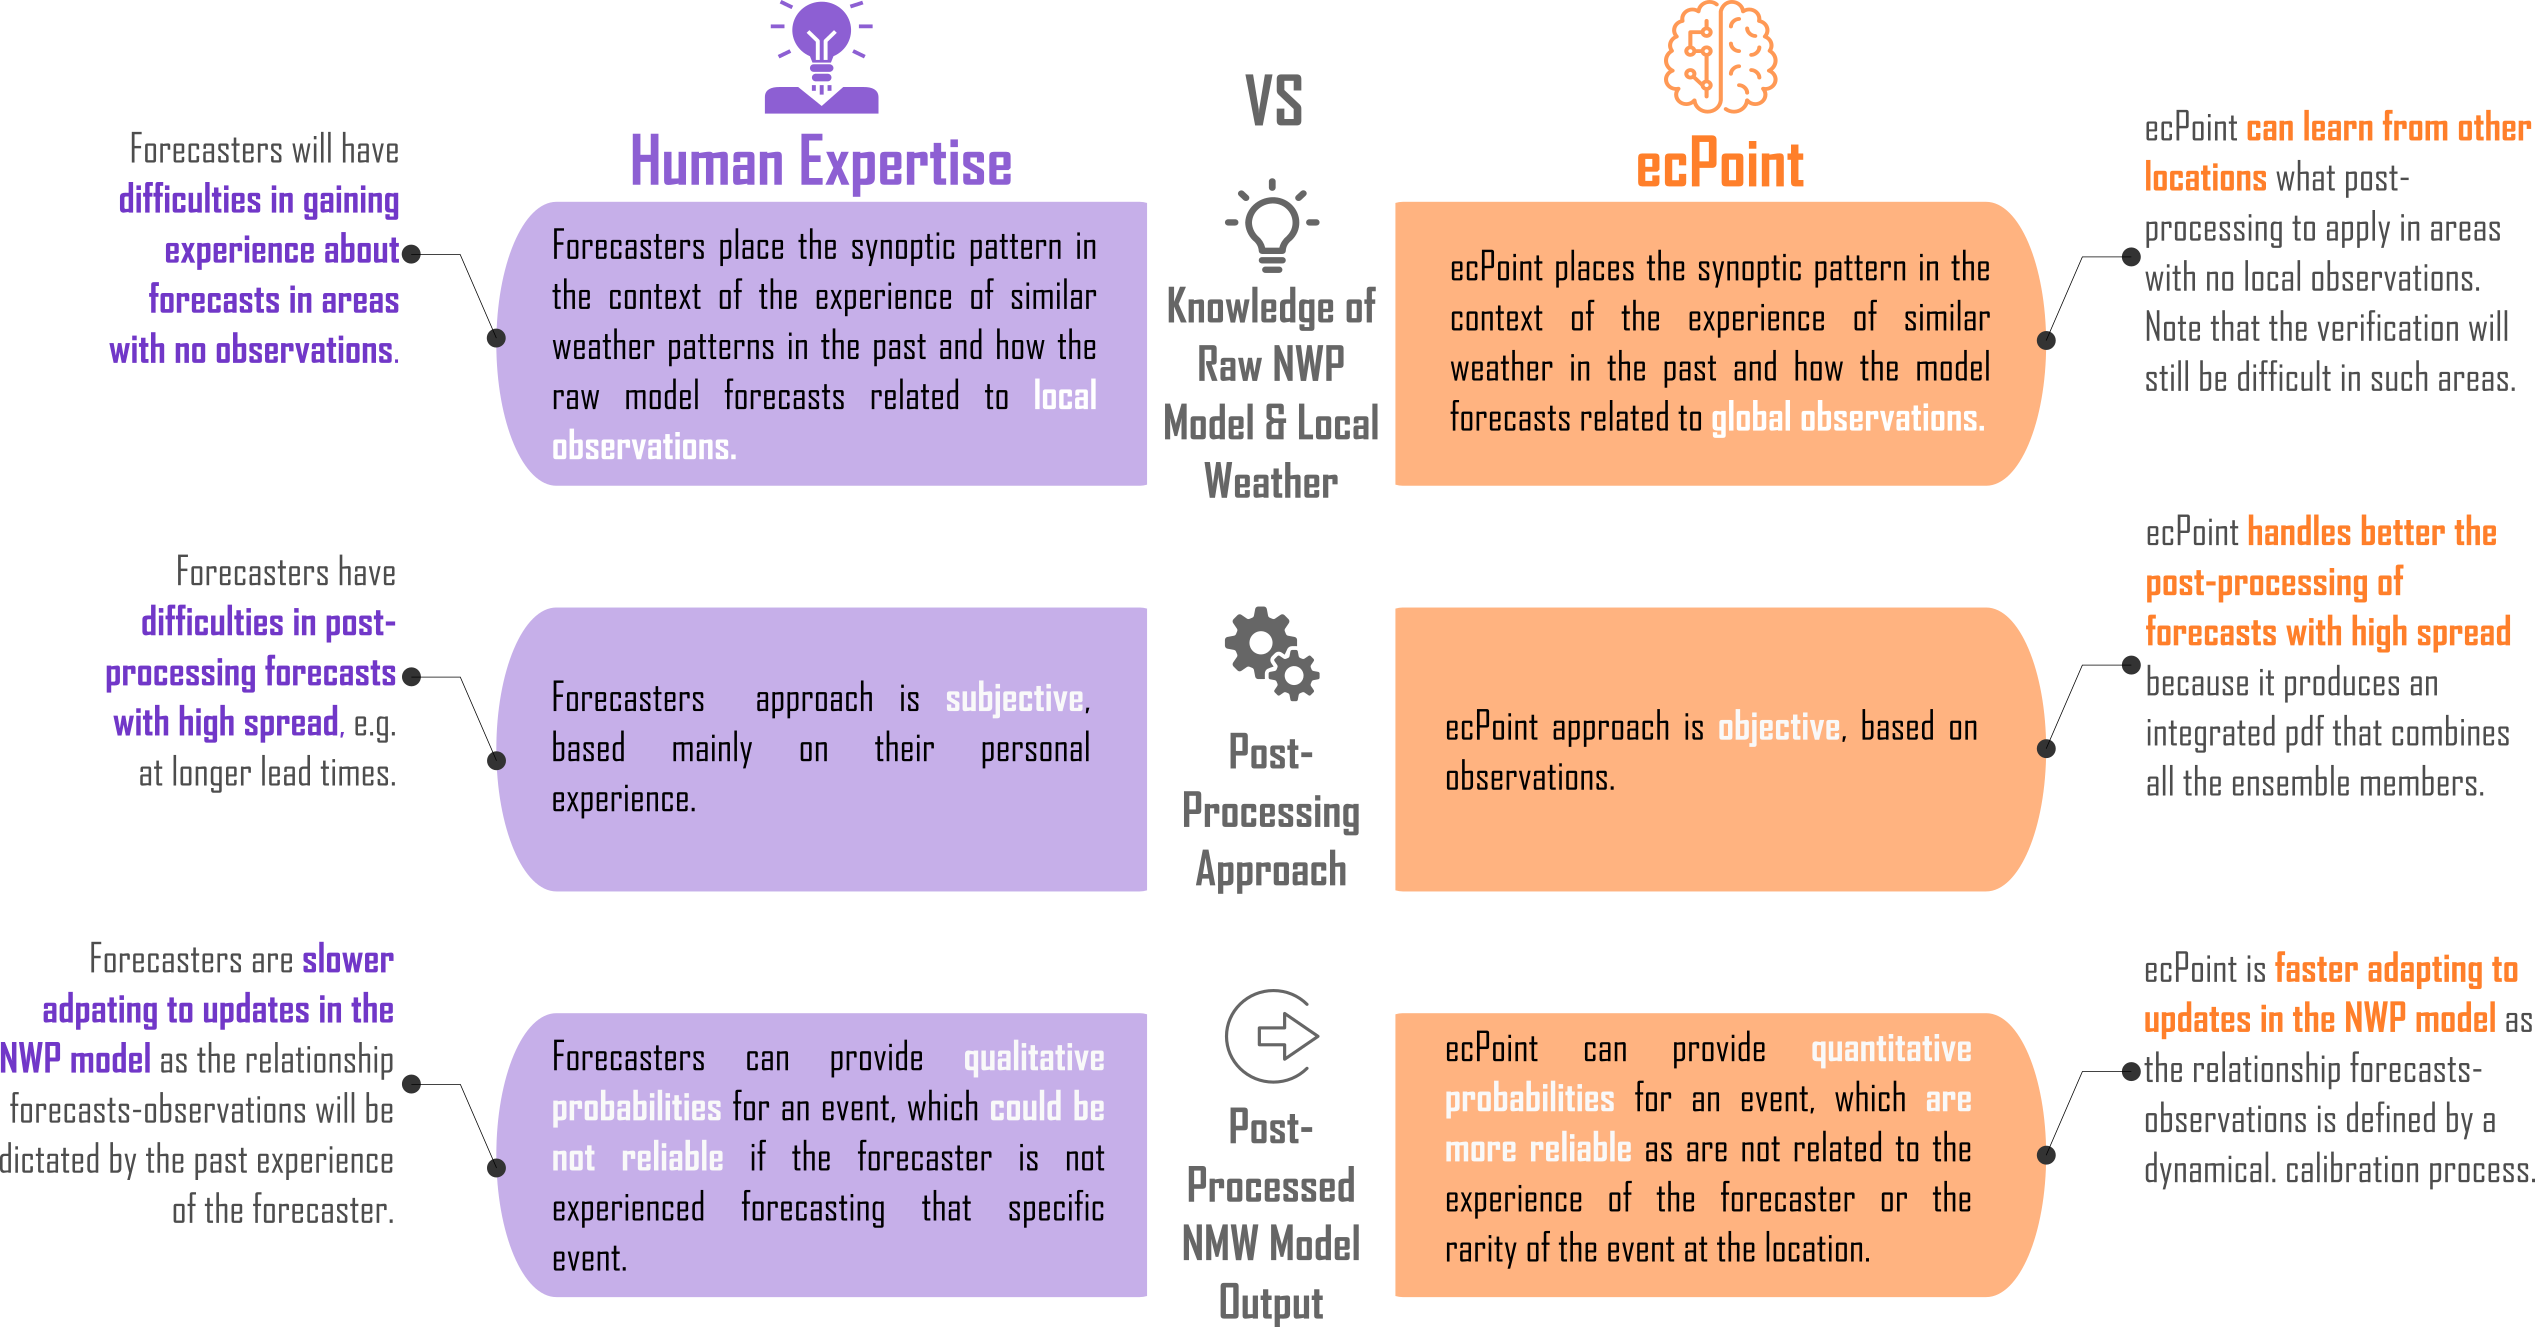
\includegraphics[width=39pc]{manuscript/Figures/Fig9.png}}
\caption{Comparison of approaches for forecasts adjustments: expert human adjustment vs. ecPoint.}
\label{Fig.9}
\end{figure*}


ECMWF continuously updates end-user needs and feedback through annual user meetings, training sessions or direct feedback, ensuring that resulting forecast products are more readily understood by recipients and integrated into their operational environments. Such request of feedback was considered even more critical for ecPoint-Rainfall as it adds layers of complexity to traditional EPS products and its outputs risk to be misunderstood if proper training is not provided. Hungary and Costa Rica volunteered to test ecPoint-Rainfall performance in predicting high-impact extreme rainfall events over a one-year trial period. Both countries decided to base their analysis on case studies. Based on the information collected on how operational forecasters used the post-processed rainfall products, this study also wants to outline some best practices when using ecPoint-Rainfall.  


\subsection{The role of forecasters in adopting new products}
Operational forecasters are the last link of a complex chain through which they transfer to society the benefits of the continuous advances in atmospheric sciences, and every scientific development would eventually affect their work.

On the one hand, some aspects of the forecasters' operational work do not help to keep up with the dynamism of developers. Among others, shift work and that many forecasters carry out their work alone or in very small groups and in periods outside office hours (nights, holidays,weekends, holidays, etc.). All these factors both slow down the adoption of new tools and the knowledge of its particularities. Another important aspect is that the added value of operational forecasters is built by cognitive processes by which the predictor recognizes atmospheric patterns and relates them to conceptual models they know or to past atmospheric situations. This requires some stability as regard to the working methodologies, tools and action protocols. This classic conception of added value has evolved as the reliability of numerical models has increased in time. The predictor's work spread to the role of intermediary between the models and the really expected weather conditions on their are of influence, acting as a translator of the model,doing a kind of human downscaling, for example, considering their systematic biases, questioning and correcting the models at key moments, also based on their experience (add Norwegian forecasters' comments).

The probabilistic approach in meteorology has imposed throughout the last years, both in modeling and in many tools and products. Thus, operational forecasters have incorporated such approach into their daily practice. However, the advances in the communication of uncertainty between different user groups have been more limited. The feeling is that the uncertainty «stays in house". This shows that the predictor is not the only part that resists changes: for example many specialized users are not aware of the usefulness of the uncertain in its decision-making processes, despite the fact that they often do use probabilistic information in other areas. 

Since the emergence of computers in operational meteorology, forecasters have counted on a fan of tools and models at their fingertips to help them in their work. Each forecaster develops its own methodology to process and handle all that information, and be able to see the forest and not just the trees. In time, number of tools and numerical models within the reach of operational forecasters have continuously increased. There is no doubt that the increased availability of models, each with their weak and strong points, has allowed to improve the quality of predictions. On the other hand, the complexity of the process of taking decisions has also increased proportionally. The more models must be handled, the more difficult it is for the forecaster to know them in depth. In addition, the frequency of updating and improving the models have also been increasing during recent years, so the predictor, which previously might be able to correct the biases of a model based on the mere experience of its use, today might not get to develop such experience before a next model version gets implemented. For example, km-scale models cannot be interpreted in the same way than global models. These high-resolution models can provide valuable information at times but in many other cases can lead to failed forecasts and false alarms, without the predictor having the time to adapt to such new models, and distinguish those cases.

Most work tools available to the operational predictor are the result of the work of meteorology professionals outside the operational environment. "Developers" tend to focus most in theoretical physical concepts, they have a deep understanding of numerical prediction and broad skills outside of strict weather(programming, etc). On the other hand, operational forecasters focus their interest on the most practical aspects, usually have very general knowledge about the numerical model but much more experience in quick decision-making processes combining different sources of data, personal experience and intuition. If initiatives aimed to increase the interaction between both groups, the prediction as a whole would benefit. The predictor would get a direct information on the characteristics of the models and the tools developed for prediction, which could be very useful to improve its exploitation. On the other hand, the "developer" could also benefit from more "real" contact with what the models seek to predict and know the needs of its direct users.


\subsubsection{The role of ecPoint-Rainfall in subjective bias-correction and downscaling raw EPS guidance}



\subsection{Hungary and Costa Rica have a fundamental different general approach to EPSs.} 
    Hungary has much longer experience with EPSs, and following the recommendations of the ECMWF Forecaster’s User guide (Owens and Hewson, 2018), their guidance on extremes is based mainly on EPS products. The latter are also disseminated to dependant centres and the public. On the contrary, Costa Rica has a shorter experience with EPSs. At short ranges, forecasters prefer greater certainty about what is going to happen locally. Such information is traditionally not provided by EPSs due to their typical coarse spatial resolutions. Ensemble products are therefore mainly used internally to assess the uncertainty of in-house forecasting systems outputs, which run at much higher spatial (typically, at km-scale) and temporal resolution (usually, at hourly scale). 

\subsection{Generalising, meteorological services with different experiences on EPSs might have different speeds in incorporating ecPoint-Rainfall products in their operational environments.}
    Such different experience on EPSs is reflected mainly by a better understanding of standard ensemble products and which one of those or which combination of those would be better to use depending on the forecaster goal. Furthermore, meteorological services with a more extended experience on EPSs might have a more efficient organisational structure to easily incorporate a wider variety of ensemble products into their operational environments. Therefore, the combination of these factors might allow better assimilation of new ensemble products, a better understanding of the underlying differences compared to other (more traditional) ensemble products, and more targeted product development to highlight such differences. For example, Costa Rica did not use to compute other than probabilities of precipitation as such product was already contained in the WRF suite. Such a product would not help forecasters in the prediction of extremes. Therefore, more initial assistance was provided (via email) to Costa Rica on what kind of products could be developed from ecPoint-Rainfall to predict extremes. Such help was not supplied to Hungary. They indeed provided autonomously a wide variety of products for ecPoint-Rainfall that would also compare raw ECMWF outputs. It is worth noticing that Costa Rica would not have been able to provide such products as they do not have access to that data.  

\subsection{Whatever products are available, local expertise and nowcasting still have a crucial role in judging those weather conditions that might trigger extreme events.}
    Unfortunately, such an approach decreases the warning lead times significantly. Ensemble forecasts could be used to increase such lead times as they highlight the forecast uncertainty. However, as highlighted in point (a), the willingness to do so depends mainly on the previous experience with EPSs.  

\subsection{Hungary and Costa Rica would use ecPoint-Rainfall at medium-range as a “pre-alert” product to increase earlier detention of extreme rainfall events and accelerate decisions on issuing warnings.}
    The overall perception from Hungary and Costa Rica is that ecPoint-Rainfall can provide useful guidance in the prediction of localise extreme rainfall, even up to medium ranges. However, as a general rule, warnings for extreme rainfall are issued no earlier than 1 or 2 days in both countries. That approach notwithstanding, they could consider using the post-processed rainfall products to increase of one or two days the warning lead times.  

\subsection{However, a fully integrated use of ecPoint-Rainfall in their operational environments is subject to the full familiarisation of the forecasters with the new post-processed product.}
    Forecasters welcome new products. However, due to lack of time as a consequence of their operational duties, it is challenging to allocate time to familiarise with new products. Thus, someone internally has to prepare easy-to-understand products and write clear documentation to make them usable for forecasters in a short time.  

\subsection{Hungary and Costa Rica feedback are useful also to understand where ecPoint-Rainfall can be improved.}
    Guidance on already know ecPoint-Rainfall weaknesses is already provided in the ECMWF Forecaster’s User Guide (Owens and Hewson, 2018). However, user’s feedback can draw on local expertise to target further research and developments. Such feedback can (1) suggest new predictors to add in the calibration, (2) identify geographical regions where the post-processed forecasts show weaknesses, and (3) pinpoint weather scenarios that are known to be problematic in raw NWP models and post-processing could improve. Users’ feedback is also helpful to assess whether it might be needed to provide additional information to the already disseminated forecasts. For example, Costa Rica expressed the will to identify whether a rainfall event is mainly convective or large-scale. Such information cannot be drawn from the currently disseminated forecasts but, instead, it could be extracted from the grid-box weather types, which are routinely computed and stored for internal forecast’s diagnosing but are not distributed to end-users. From the feedback collected from Costa Rica, it seems though that such information could be beneficial for end-users. 
    
\subsection{A more direct contact with users in the initial stages of product release is needed to ensure a correct interpretation of ecPoint-Rainfall products.}
    How to interpret and communicate probabilistic forecasts is a very well-known problem within the scientific community  (Cloke and Pappenberger, 2009; Demeritt et al., 2013; Ramos et al., 2010). It is considered that this is even more true for ecPoint-Rainfall as it adds complexity to standard probabilistic forecasts. This study has identified a need for specific training when working with ecPoint-Rainfall, whatever is the previous experience with EPSs, to avoid any misrepresentation of the new probabilistic product. The choice of both Hungary and Costa Rica to develop a product to identify extreme rainfall events based on the 85th percentile is a prime example. Such percentile might seem suitable to provide guidance on extremes, but two main points should be considered. Firstly, the 85th percentile represents the crossing point between raw ECMWF and post-processed rainfall forecasts, so the user would not be taking advantage of the additional information provided by ecPoint-Rainfall. Secondly, the 85th percentile represents a value that has a 1 in 7 chance to be exceeded. The new product aims to forecast very extreme localised rainfall, which typically has a much lower occurrence probability, typically 1 in 20 or 1 in 100 chance. To capture such events, therefore, it would be more appropriate to look at higher percentiles, such as 98th or 99th, as shown in the discussion of the case studies.  Another prime example given by Costa Rica is the wrong interpretation of what is possible to forecast with ecPoint-Rainfall. In point (a) it was highlighted that Costa Rica would prefer to use km-scale NWP models at short ranges as they would like to have greater certainty on what might happen locally. They said that they did not use ecPoint-Rainfall for this scope. However, this is precisely what the new post-processed product should be used for. Unfortunately, this essential aspect of ecPoint-Rainfall was missed or misunderstood. ecPoint-Rainfall is indeed disseminated on the same grid of the raw ECMWF ensemble. However, they do not operate on the same spatial scale. Raw ECMWF ensemble provides an average of the point rainfall values that might be observed within the grid-boxes. ecPoint-Rainfall, instead, forecasts rainfall values that might be observed at a point within the raw ensemble grid-box, even though it is not possible to say where such point-wise value might occur within the grid-box. 


%%%%%%%%%%%%%%%%%%%%
% Conclusions
\section{Conclusions and Future Work}
This work aimed to understand whether the "standard" user guidelines for communicating the meaning and the use of "standard" probabilistic forecasts would be suitable to deliver the added benefits of the new probabilistic ecPoint-Rainfall forecasts. The answer is yes, and no. On the one hand, it is not necessary to reinvent the wheel, while on the other side not only ecPoint-Rainfall have raised the bar on predicting rainfall at points more skillfully and reliably, but also in communicating its forecasts. It highlights, more than any other severe-weather-oriented probabilistic product, how important it is to convey the shades of grey to users, who otherwise might see ecPoint-Rainfall outcomes only as black or white. Once this is understood, it will be possible to create tailored user guidelines that will facilitate the extraction of the full potential of the new product and will address the needs of users with different levels of knowledge on probabilistic weather forecasting. The latter aspect is probably the most important in the whole paper. If users who do not use probabilistic forecasts, because such forecasts are considered not reliable, are reached by the message that ecPoint-Rainfall fulfill most of their needs (as opposed to standard probabilistic products), it might be possible to increase the catchment of users of probabilistic products exponentially.
The strong under-prediction bias for large localized totals as historically be an impediment to the uptake of global probabilistic forecasts by those users whom this aspect is of paramount importance.


%%%%%%%%%%%%%%%%%%%
% ACKNOWLEDGMENTS %
%%%%%%%%%%%%%%%%%%%
\acknowledgments
We thank the anonymous reviewers, Florian Pappenberger, David Richardson who helped to improve the manuscript with their comments.


%%%%%%%%%%%%%%%%%%%%%%%%%%%%%%%
% DATA AVAILABILITY STATEMENT %
%%%%%%%%%%%%%%%%%%%%%%%%%%%%%%%
\datastatement
The data that support the findings of this study are available from the corresponding author upon request.


%%%%%%%%%%%%%%
% REFERENCES %
%%%%%%%%%%%%%%
\bibliographystyle{ametsoc2014}
\bibliography{references}

\end{document}